\section{Base di dati sistema coordinazione}

\subsection{Abstract}

L'obiettivo è quello di sviluppare un sistema che coordini e decida quando illuminare o non illuminare specifiche zone. Questo sistema dovrà tenere traccia di tutte le informazioni relative allo stato attuale dei lampioni.

Il sistema si collegherà ad altre componenti esterne, utilizzando algoritmi proprietari, e deciderà quando effettuare cambiamenti di stato. Si consiglia la visione del capitolo \ref{cap:sistema-coordinazione}.

\subsection{Analisi dei requisiti}

\subsection{Progettazione concettuale}

\subsubsection{Analisi delle entità}

\textbf{Se non specificato l'attributo è NOT NULL}

%LAMPIONE
\begin{center}
    \begin{tabularx}{\textwidth}{|l|l|l|X|}
        \hline
        \rowcolor{gray!30}
        \multicolumn{4}{|c|}{\textbf{LAMPIONE}}\\
        \hline
        id & INTEGER & Identifica univocamente un lampione all'interno del sistema & Chiave\\
        \hline
        luminosita & INTEGER & \multicolumn{2}{l|}{Livello di luminosità in cui si trova il lampione} \\
        \hline
        istanteUltimaModifica & LONG & \multicolumn{2}{l|}{Indica quando c'è stata l'ultima variazione di luminosità ad un lampione} \\
        \hline
    \end{tabularx}
\end{center}

\subsubsection{Schema ER concettuale}

\begin{center}
    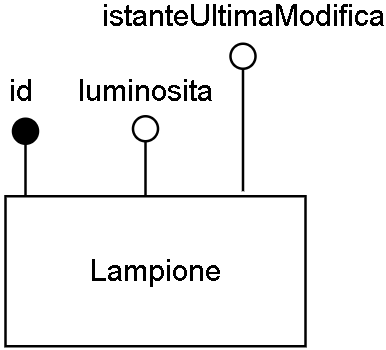
\includegraphics[width=4.5cm]{contenuti/specifica-basi-dati/img-sbd/coordinazione_concettuale.png}
\end{center}

\subsection{Progettazione logica}